\chapter{Spatio-temporal modeling of PSI displacements}

\begin{figure}[H]
\begin{center}
		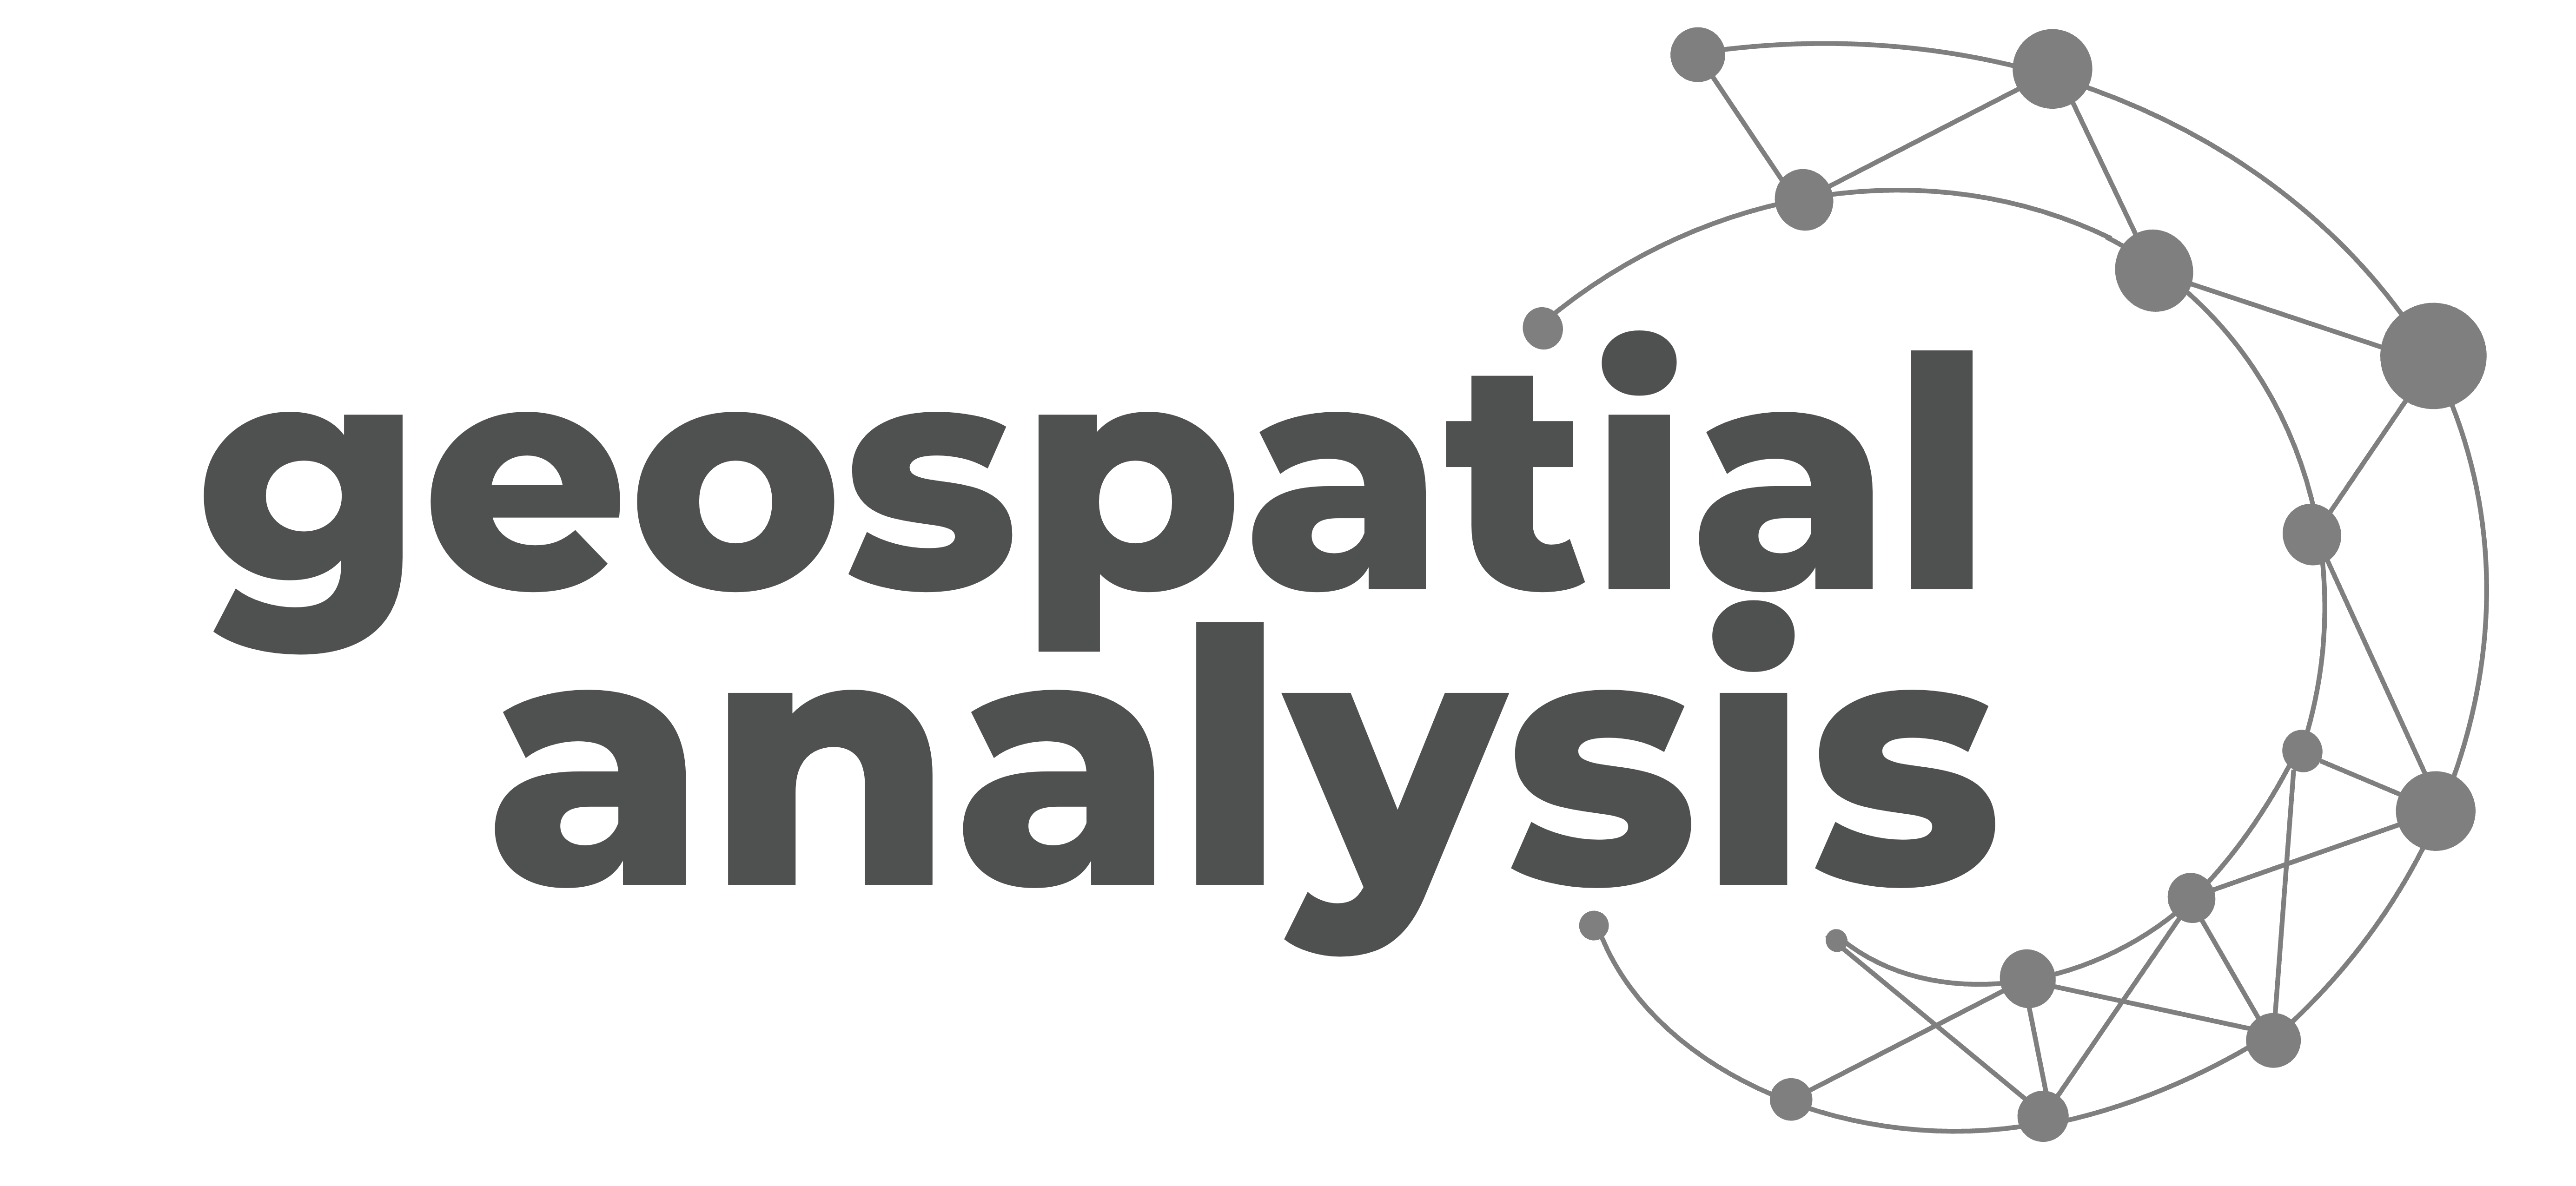
\includegraphics[width=0.8\columnwidth]{images/PHASE_mod2.png}
\end{center}
\end{figure}

\section{Preliminary steps}

The \textbf{Displacement Modeling} section of the PHASE hub performs interpolation and modeling of PS time series generated by StaMPS PSI. It can also use externally generated PSI data when the input tables follow the expected format. Open it through the persistent hub navigation; do not copy a standalone \texttt{.mlapp} into a project.

The application requires MATLAB and the Python environment configured by the PHASE installation. Report generation uses Python packages such as \texttt{openpyxl} and \texttt{pillow}; use the installer's checks and the run log to diagnose missing packages.

\begin{quote}
    \textcolor{cyan}{\textbf{SUGGESTION:}} \textcolor{gray}{If Python integration fails, compare the Python interpreter shown by MATLAB's \texttt{pyenv} with the interpreter configured by the PHASE installer. Installing a package into a different Python environment will not fix the active runtime.}
\end{quote}

\noindent Some geospatial modeling operations can be highly computationally expensive. If the execution takes too long or exceeds your system's memory, you should try reducing the spatial resolution of the requested output grid.

\begin{quote}
    \textcolor{orange}{\textbf{WARNING:}} \textcolor{gray}{Please remember that all provided InSAR displacements are measured strictly along the satellite Line-of-Sight (LOS), which is a 1D vector.  The software models this specific 1D deformation and does not inherently decompose it into true vertical or horizontal 3D vectors.}
\end{quote}

This module of PHASE requires the following MATLAB packages to be installed:
\begin{itemize}
    \item Curve Fitting Toolbox.
    \item Image Processing Toolbox.
    \item Mapping Toolbox.
    \item Optimization Toolbox.
    \item Parallel Computing Toolbox.
    \item Signal Processing Toolbox.
    \item Statistics and Machine Learning Toolbox.
\end{itemize}

\section{Required folder structure}

PHASE code remains in the shared installation. Select or create a project in the hub, open \textbf{Displacement Modeling}, and point the module at the desired PSI output within \texttt{03\_RESULTS} (or at a compatible external dataset). Modeling output belongs to the project results area. Existing projects may use their original folder names.

\section{Description of the MATLAB application}
This stage takes scattered PS time series generated by StaMPS PSI (or external PSI processors) and converts them into temporal or spatio-temporal models and reports. The scientific options below remain relevant to the version 7 module; control placement may differ slightly from older PHASE releases.

\subsection{Input files}
Select the PSI output spreadsheet (\texttt{.xlsx} or \texttt{.csv}) and confirm the Python interpreter if prompted. For PHASE-generated series, check the adjacent \texttt{\_series.json} metadata so that you know whether the input is Standard \texttt{v-do}, TRAIN-corrected \texttt{v-dao}, or Step 8-corrected \texttt{v-dso}; these are scientifically different inputs.

Additionally, the date of the first observation in the time series must be specified. There is also a checkbox to automatically remove all the previous output folders prior to the software execution.


\subsection{Area of interest}
The second step involves defining the AOI, which delineates the spatial boundaries for computing and modeling displacements. This AOI can be specified on the map or by a shapefile. A shapefile must include a readable \texttt{.prj} defining WGS84 geographic coordinates or a WGS84-based projected CRS; coordinates are never guessed from their numeric range. PHASE projects the AOI, PS and optional query points into one common UTM CRS. If the AOI crosses two adjacent UTM zones, it chooses the zone covering the larger part of the AOI. Very wide, polar, equator-crossing and antimeridian-crossing AOIs require a different projection and are rejected explicitly rather than processed with inconsistent coordinates. Points outside the AOI are filtered to focus processing only on relevant PS.


\subsection{Processing options}

Depending on your analytical needs, the application allows you to choose between two alternative main processing modes, both of which conclude with automatic report generation:

\begin{description}[style=nextline]
    \item[Alternative 1: Temporal-only modeling (PS-by-PS)]
    This mode focuses strictly on the time domain without performing any spatial interpolation between points. The software automatically cleans and mathematically decomposes each individual PS time series. This includes: outlier removal, low-degree polynomial trend estimation, Fourier-based periodicity analysis, spline-based modeling of residual local components, and stochastic collocation on the residuals.

    \item[Alternative 2: Spatio-temporal modeling (interpolation)]
    This mode performs a joint spatio-temporal modeling, taking the scattered points data and interpolating them into continuous displacement fields. You can choose between two mathematical approaches (Deterministic splines or Stochastic Least Squares Collocation) across two spatial domains:
    \begin{itemize}
        \item \textbf{1D domain:} used when monitoring linear structures defined by a centerline (e.g., roads, railways, narrow arch dams).
        \item \textbf{2D domain:} used when monitoring wide, areal targets (e.g., cities, landslides, earth-filled dams).
    \end{itemize}

    \item[Final step: Automatic reporting]
    Regardless of which modeling path you choose, the module finalizes the process by generating a comprehensive Excel report (via Python integration) and reproducible, publication-ready maps. It also automatically applies thresholding to highlight specific areas exhibiting anomalous displacement behavior.
\end{description}

The overall flow of these processing options is schematized in the figure below.

\begin{figure}[H]
    \centering
    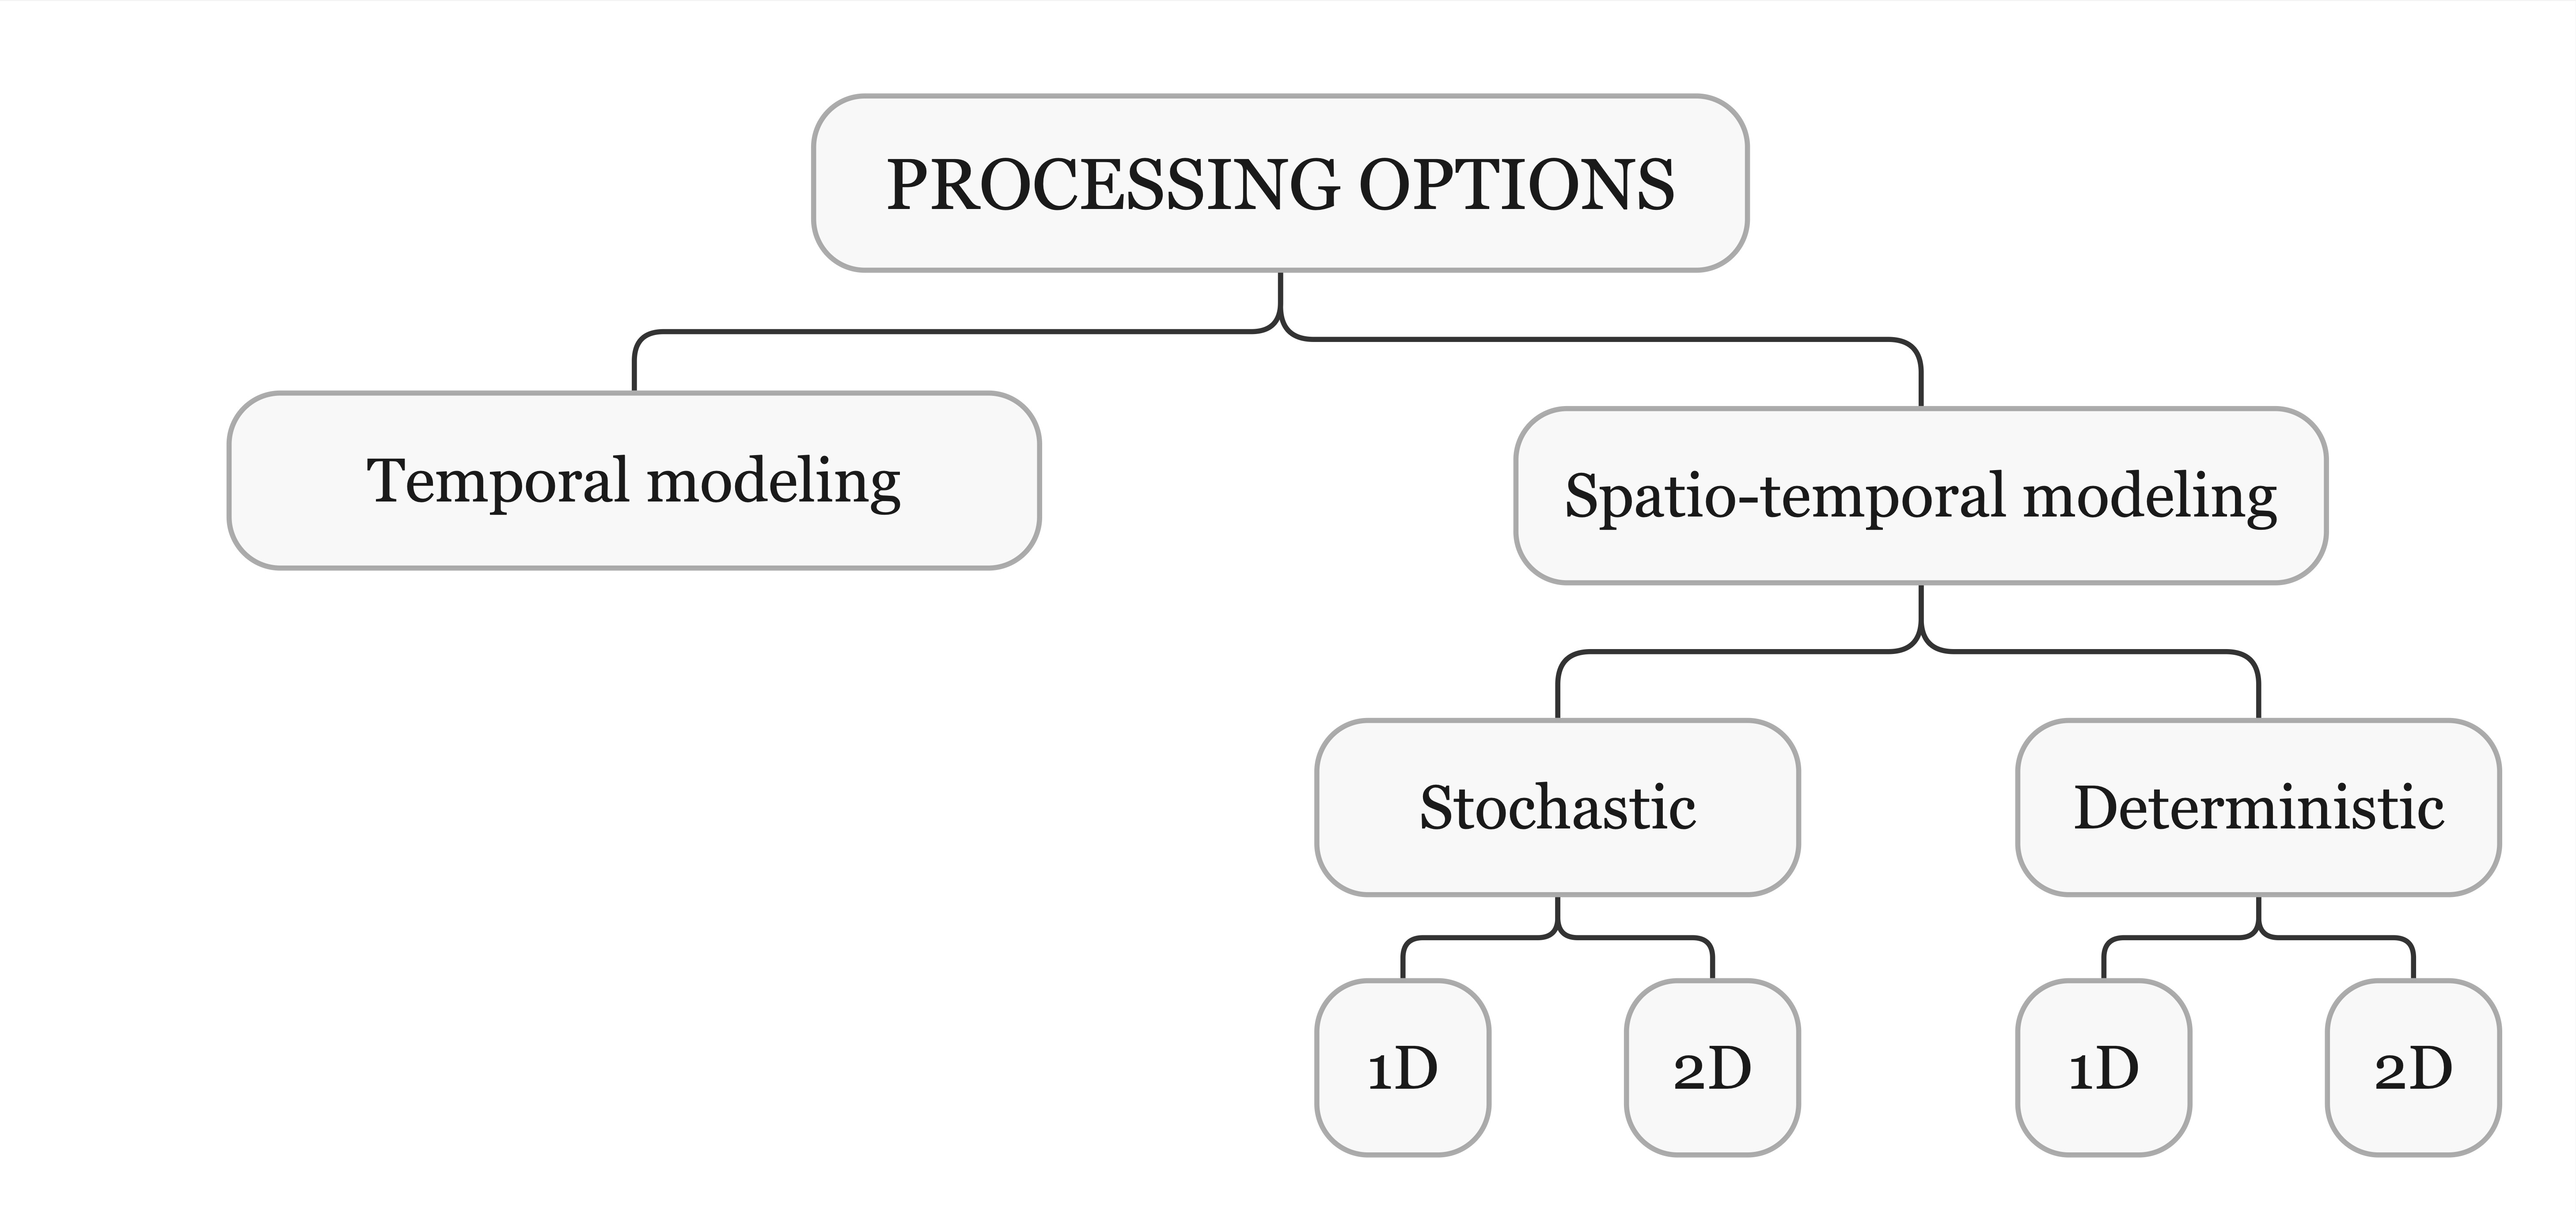
\includegraphics[width=0.9\textwidth]{images/Processing_options.jpg}
    \caption{Schematic representation of the processing options available in PHASE.}
\end{figure}

Consequently, the GUI has 4 available processing types:
\begin{itemize}
    \item \textbf{Temporal}: interpolation of all time series independently.
    \item \textbf{Temporal\&NNI}: interpolation of all time series independently and nearest neighbor spatial interpolation for visualization.
    \item \textbf{Spatio-temporalDET}: spatial interpolation with deterministic methodology.
    \item \textbf{Spatio-temporalSTC}: spatial interpolation with a joint deterministic and stochastic methodology.
\end{itemize}

\begin{figure}[htbp]
    \centering
    
\includegraphics[width=\textwidth]{images/Screenshot 2026-10-11 alle 23.11.56.png}
    \caption{Model design in the PHASE 7 Displacement Modeling section. The example selects a two-dimensional spatio-temporal stochastic model; blank and unsaved controls in the screenshot are not a configuration to run as-is.}
    \label{fig:phase7-model-design}
\end{figure}

The following subsections explain how to configure each tab in the GUI.


\subsection{Temporal modeling}\label{ss:temp}
When the user selects the temporal-only mode, Module 2 performs a fully automated decomposition of every individual PS time series. The objective is to separate the physical deformation signal from background noise by modeling each scatterer independently, without influence from neighboring points.

\subsubsection{The configuration panel}
The temporal workflow is driven by a dedicated GUI section that centralizes the user-configurable parameters.

Through this interface, users can define the core parameters that govern the underlying mathematical estimators without needing advanced statistical expertise. Key selectable options include:
\begin{itemize}
    \item \textbf{A priori noise variance model:} choose between a coherence-based model, a constant manual value, or automatic estimation from the Fourier spectrum.
    \item \textbf{Spline knot number:} allow the software to automatically estimate the number of knots via statistical methods (variance threshold, MDL, F-test, $\chi^2$ test), or define them manually.
    \item \textbf{Regularization strength:} set the smoothing parameter $\lambda$ for the spline fit (automatic or user-defined).
    \item \textbf{Collocation strategy:} choose between filtering (estimation strictly at observation points) or prediction (interpolation).
    \item \textbf{Centerline/grid resolution:} define the resolution of the regular spatial domain for the estimation (\textit{available only if NNI is selected}).
\end{itemize}


\subsubsection{The processing workflow}
Once initiated, the software processes each PS through five sequential core stages, plus one optional spatial visualization stage.

\begin{figure}[H]
    \centering
    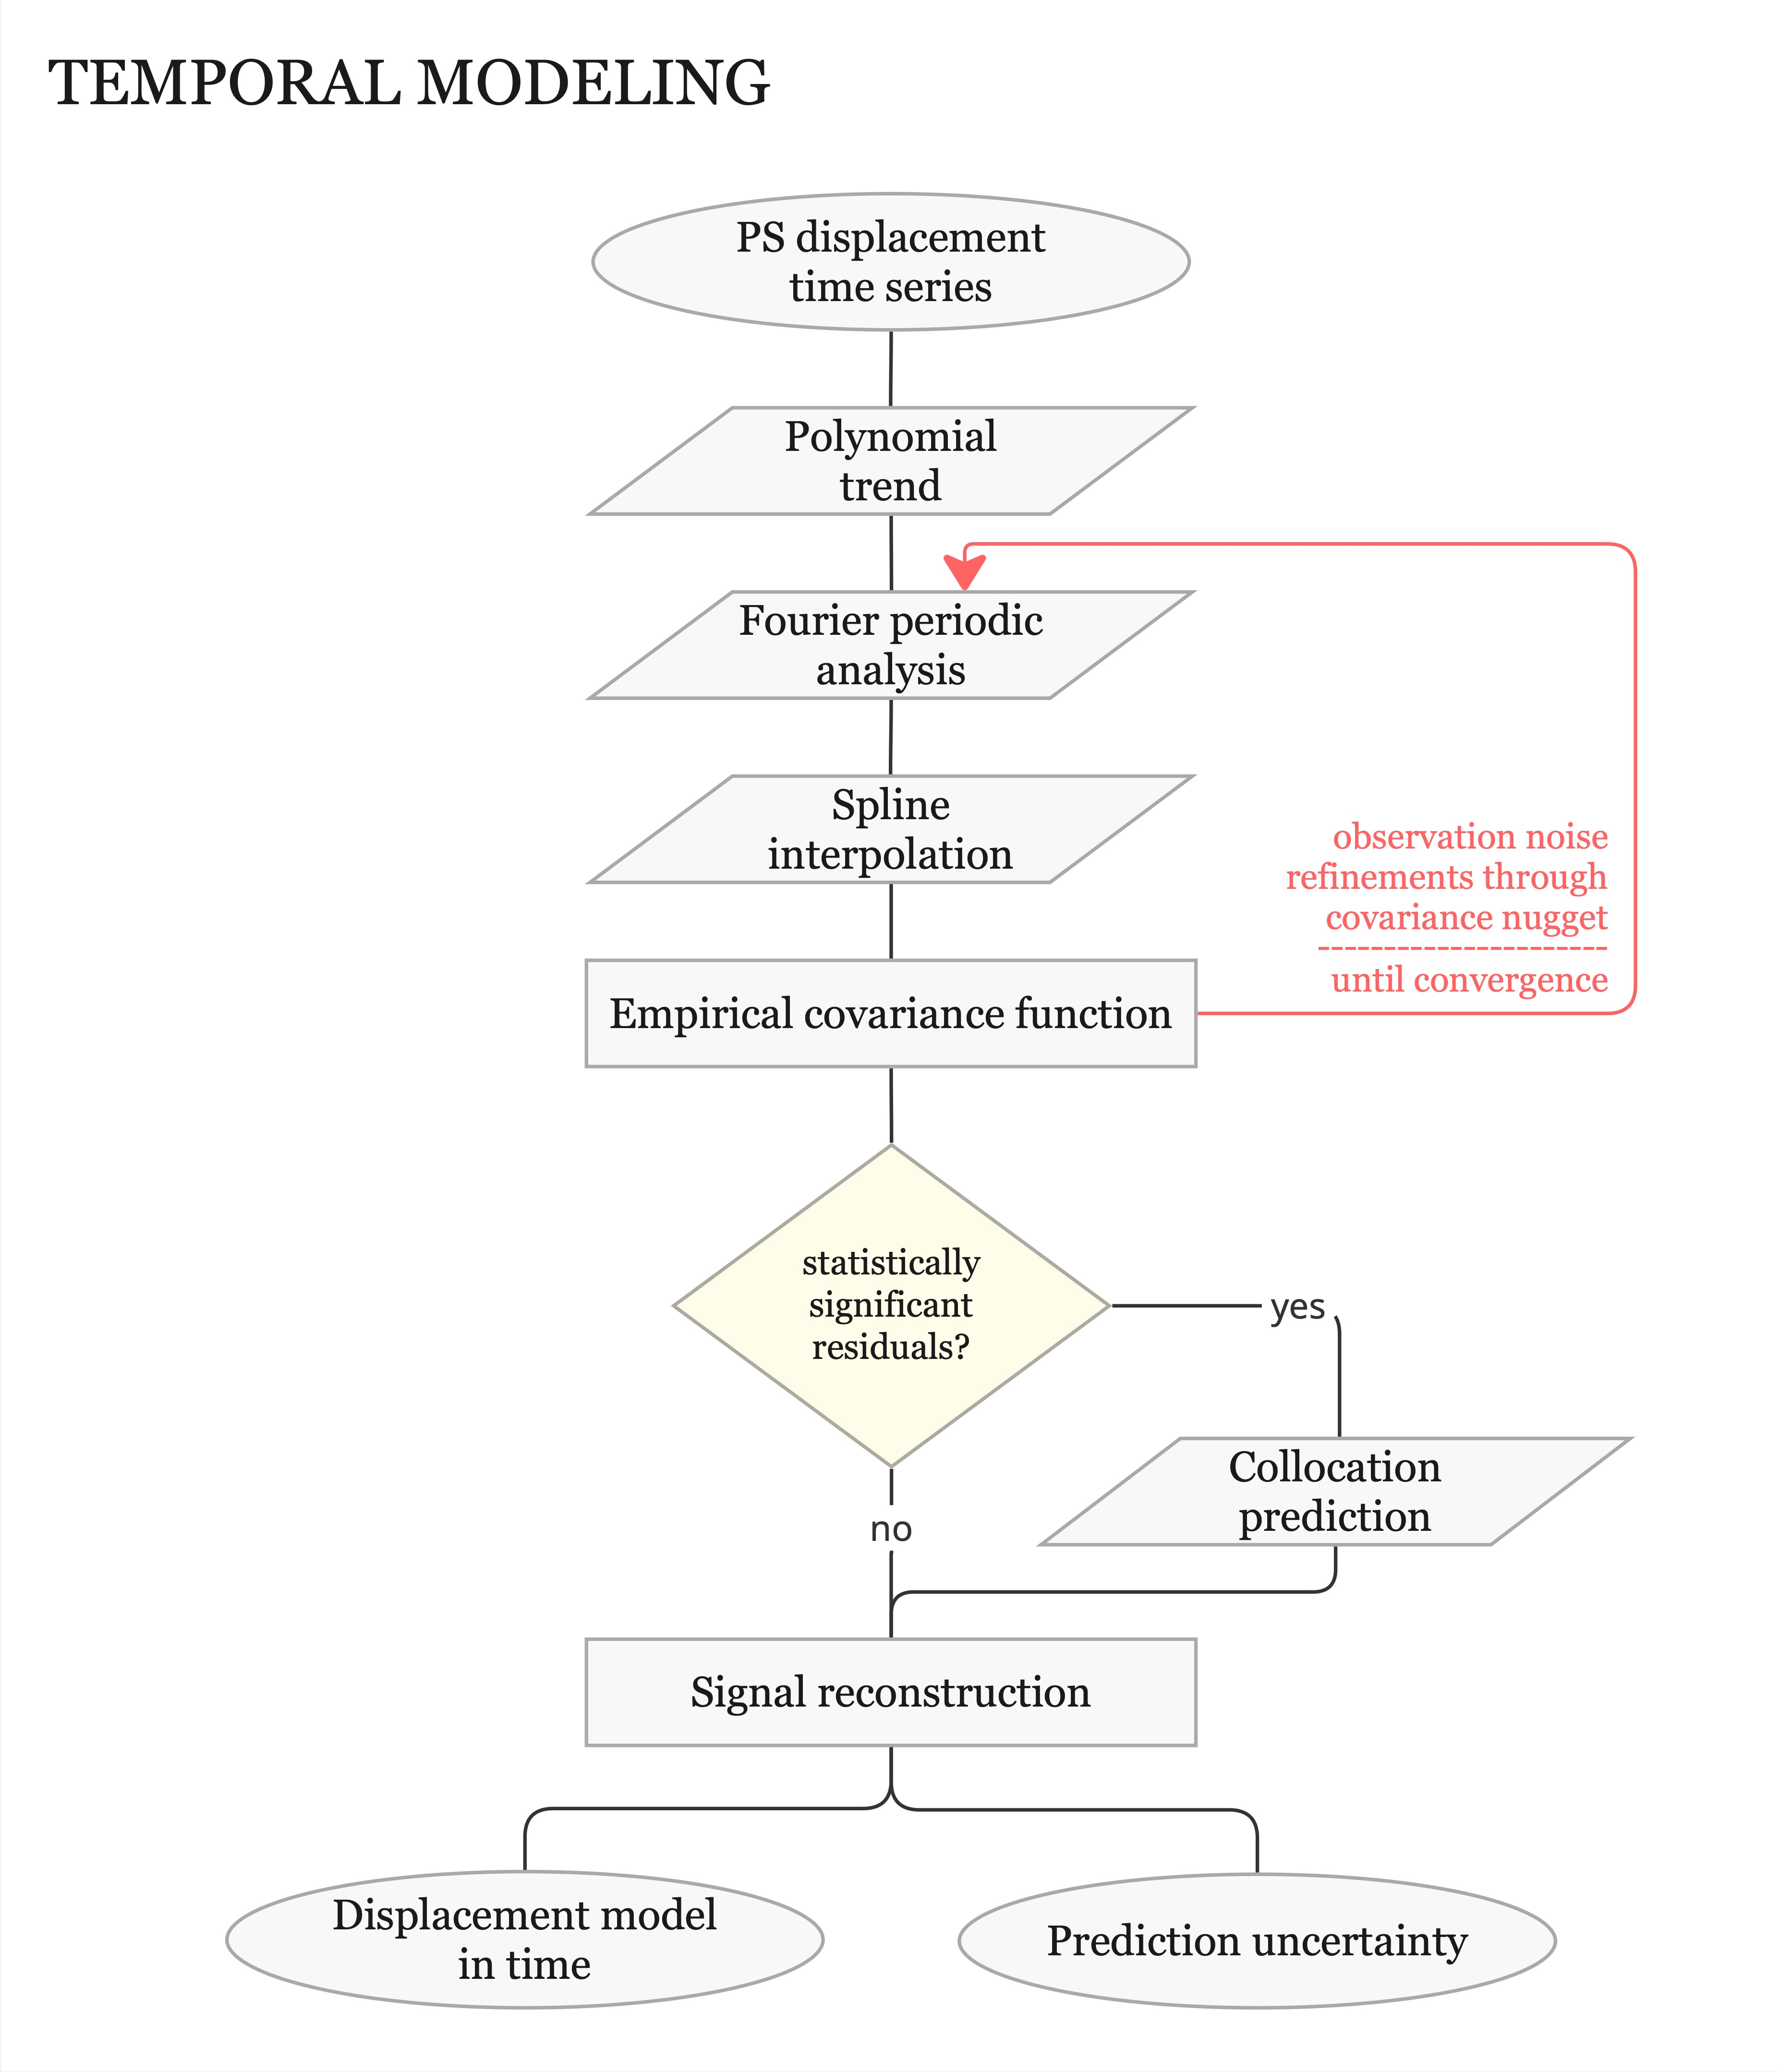
\includegraphics[width=1\textwidth]{images/G_temporal_modelling.jpg}
    \caption{Schematic representation of the temporal modeling workflow. Each PS time series is decomposed into deterministic, periodic, local, and stochastic components.}
    \label{fig:temporal_workflow}
\end{figure}

\begin{enumerate}
    \item \textbf{Deterministic trend estimation:} isolates the long-term linear or polynomial deformation component.
    \item \textbf{Periodic/seasonal analysis:} identifies and isolates cyclic thermal or seasonal oscillations.
    \item \textbf{Local modeling with splines:} captures non-linear, localized kinematic behaviors.
    \item \textbf{Empirical covariance estimation:} analyzes the residual stochastic (random) process.
    \item \textbf{Collocation:} applies filtering or prediction to obtain a smoothed, physically consistent time series.
    \item \textbf{Optional spatial visualization:} generates a quick spatial overview using Nearest Neighbor Interpolation (NNI).
\end{enumerate}

\subsubsection{Final signal reconstruction}
Because the model is built sequentially, the final reconstructed displacement estimate $\hat{d}(t)$ for any given PS is simply the sum of the isolated physical components evaluated at the target epochs:
\begin{equation}\label{eq:displ_tot}
    \hat{d}(t) = \hat{d}_{\text{trend}}(t) + \hat{d}_{\text{periodic}}(t) + \hat{d}_{\text{spline}}(t) + \hat{d}_{\text{collocation}}(t)
\end{equation}

\textbf{Understanding uncertainty:} Because each component is estimated conditionally based on the previously removed signals, you cannot simply add their individual standard deviations together. Therefore, the total uncertainty of the fully reconstructed time series $\sigma_{\hat{d}}(t)$ is represented solely by the point-wise prediction variance of the final modeled residuals.

Depending on whether the stochastic signal is physically significant enough to trigger collocation, the final reported uncertainty is defined as:
\begin{equation}
{\sigma}^2_{\hat{d}}(t) \approx
\begin{cases}
    {\sigma}^2_{\hat{d}_{\text{spline}}}(t) & \begin{array}{@{}l@{}} \text{if stochastic signal is negligible} \\ \text{(collocation skipped)} \end{array} \\
    {\sigma}^2_{\hat{d}_{\text{collocation}}}(t) & \text{otherwise}
\end{cases}
\end{equation}


\subsection{Spatio-temporal stochastic}\label{sec:1D_stc}
The stochastic approach evaluates the behavior of all PS points simultaneously. This allows the software to rigorously filter out spatially uncorrelated noise (e.g., phase unwrapping errors) and statistically interpolate data across areas lacking radar targets.

The complete procedural sequence for this stochastic spatio-temporal modeling is schematized in Figure~\ref{fig:diag_stoch}. This is valid for both 1D and 2D geometries.

\begin{figure}[H]
    \centering
    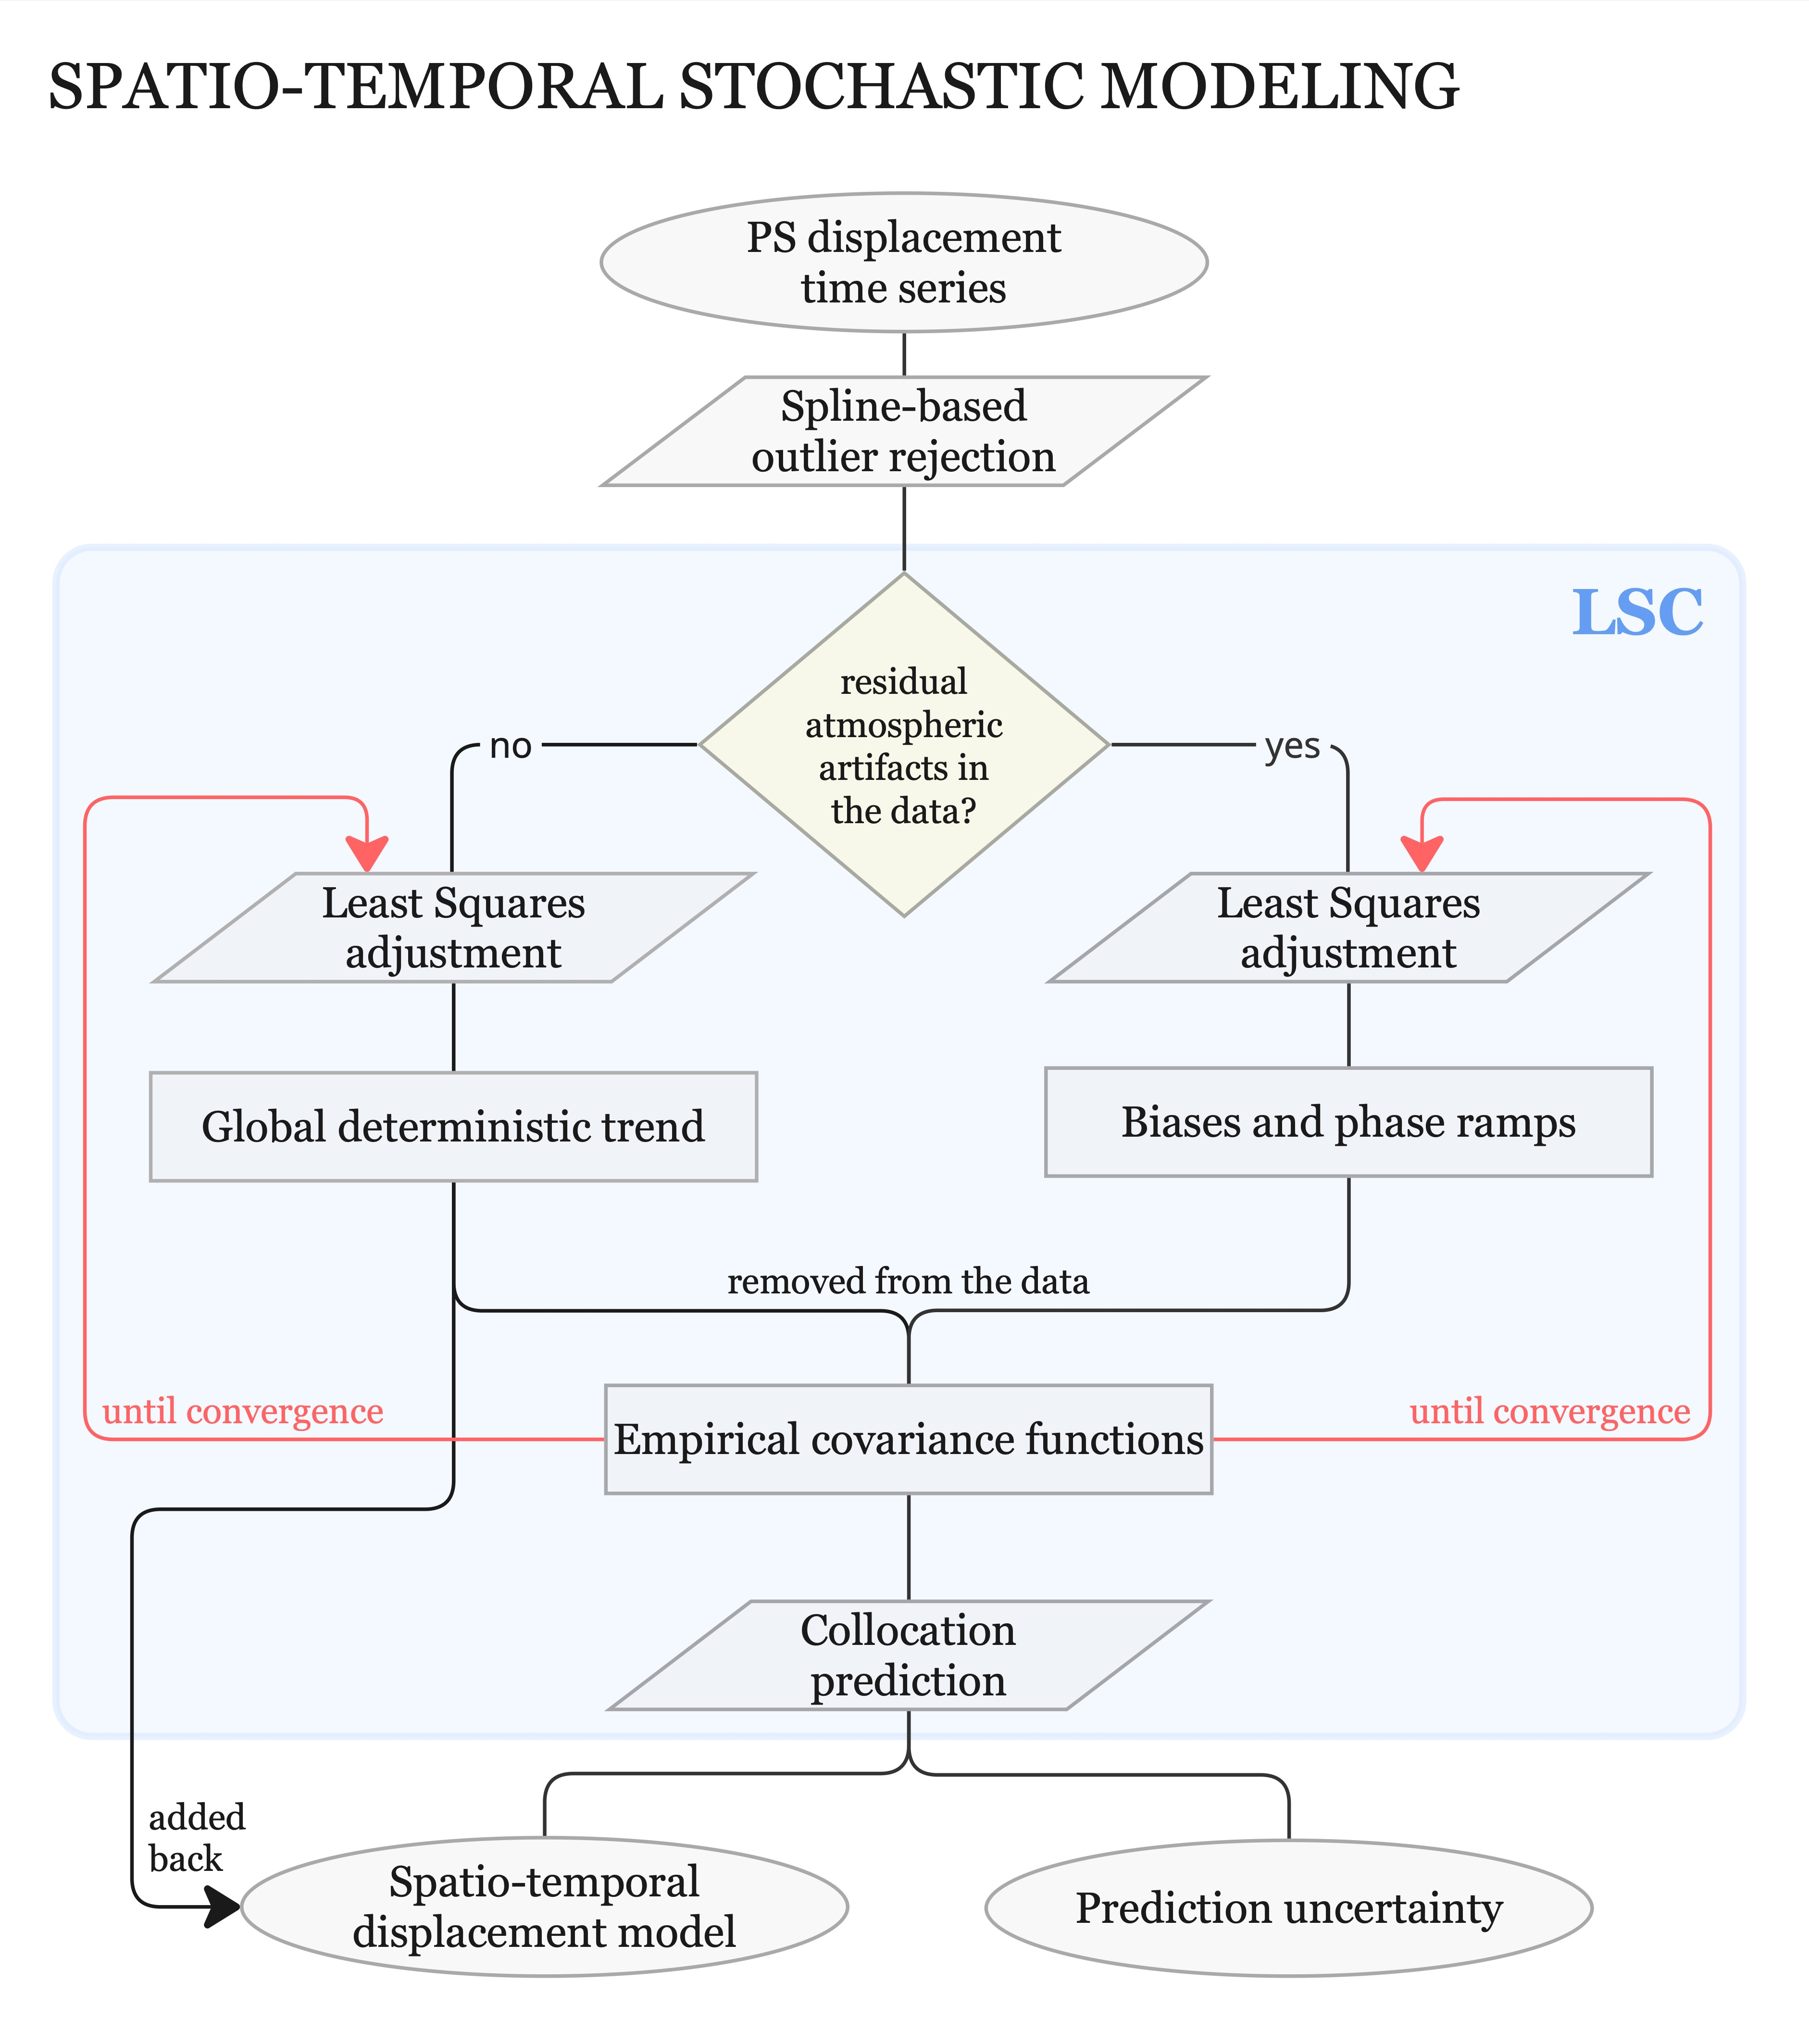
\includegraphics[width=1\textwidth]{images/G_ST_stochastic.jpg}
    \caption{Schematic representation of the stochastic spatio-temporal modeling workflow, progressing from raw PS observations through outlier rejection, empirical covariance fitting, and LSC.}
    \label{fig:diag_stoch}
\end{figure}

To facilitate the interpretation of this massive, multi-dimensional dataset, the software automatically generates dynamic and static visualizations as the final step of the processing workflow:
\begin{description}
    \item[Dynamic time-lapse (GIF):] a continuous animation is produced displaying the reconstructed displacement field superimposed on a satellite basemap. This allows users to visually track the progression of deformation phenomena throughout the entire monitoring period.
    \item[Static spatio-temporal maps:] \textit{only for 1D spatial geometry} to fit both the spatial and temporal dimensions into a single plot, the software generates 2D raster maps where the X-axis represents the curvilinear centerline coordinate ($\ell$), the Y-axis represents time ($t$), and the color scale represents the continuous displacement magnitude. An identical accompanying map is generated for the estimation uncertainty ($\boldsymbol{\sigma}_{\hat{d}}$), providing a quantitative assessment of the model reliability across space and time.
\end{description}


\subsubsection{1D spatial domain}
The workflow is configured through the 1D stochastic controls, providing access to the underlying statistical estimators without manual code modifications.

Through this interface, you govern the specific estimators used in the Least Squares Collocation framework. Key configurable parameters include:
\begin{itemize}
    \item \textbf{Centerline and time resolution:} defines the uniform spatial ($\Delta \ell^\text{out}$) and temporal ($\Delta t^\text{out}$) step sizes for the target prediction grid. This dictates the resolution of your final continuous displacement model.
    \item \textbf{Minimum period for splines fitting:} establishes the maximum flexibility of the spline curves used during the preliminary temporal outlier rejection step, preventing the algorithm from overfitting short-term noise.
    \item \textbf{Approach for LSC (Signal vs. Noise separation):} dictates how large-scale atmospheric delays and orbital errors are handled. You can choose to absorb them into the noise model, or assume clean data and fit a low-degree deterministic polynomial prior to collocation.
    \item \textbf{Atmospheric residual errors:} if present, specifies whether these errors are treated as purely time-variable biases (suitable for small AOI) or as spatio-temporal trends (required for large AOI).
    \item \textbf{Global polynomial:} defines the maximum permissible degree for the global deterministic trend fitted across the entire infrastructure axis (if assuming clean data).
    \item \textbf{Steps to average the empirical covariance:} controls the lag-binning resolution used to compute the empirical covariance point clouds. This can be determined automatically based on data density or set manually.
    \item \textbf{Covariance model:} selects the continuous mathematical function used to fit the empirical covariance data. This generates the positive-definite matrix strictly required for the final stochastic prediction.
\end{itemize}

To construct a continuous spatio-temporal deformation model along a linear infrastructure, the irregularly scattered PS observations must first be orthogonally projected onto the centerline of the element. Their spatial position is subsequently described purely by a 1D curvilinear coordinate ($\ell$), originating at the beginning of the selected segment.

\begin{quote}
    \textcolor{orange}{\textbf{WARNING:}} \textcolor{gray}{If portions of the infrastructure lack PS points (e.g., highway tunnels, which are undetectable by SAR), these sections are treated mathematically as data gaps. Because this model generates a continuous field, displacement values within these gaps are the result of pure statistical extrapolation. Always interpret extrapolated values in large data gaps with caution.}
\end{quote}

Once projected, the available displacement time series undergo a multi-step processing workflow to filter noise, remove artifacts, and prepare the data for geostatistical interpolation.


\subsubsection{2D spatial domain}
When the AOI represents a spatially distributed target---such as an urban center, a volcanic caldera, or a subsidence bowl---constraining the deformation to a 1D centerline is physically inappropriate. To address this, PHASE extends the stochastic modeling framework into a full 2D planar geometry.

The algorithmic pipeline for the 2D case is a direct extension of the 1D workflow. The mathematical estimators, outlier rejection testing, and iterative covariance updates remain fundamentally identical. The core differences lie strictly in the geometric definition of the spatial domain (incorporating the assumption of spatial homogeneity and isotropy) and the 2D expansion of the deterministic trend models.

If this approach is selected, the 2D stochastic controls become available. The parameters largely mirror the 1D configuration, with a planar spatial-resolution definition.

In the 2D domain, the \textbf{spatial and time resolution} parameter defines a uniform grid spacing applied equally to both the Easting ($x$) and Northing ($y$) coordinates, rather than a single curvilinear distance.

\begin{quote}
    \textcolor{orange}{\textbf{WARNING:}} \textcolor{gray}{Similar to the 1D case, displacement values generated over areas lacking PS points are the result of statistical extrapolation. Because 2D extrapolation expands radially across a plane, prediction uncertainties can grow rapidly in large spatial data gaps. Always interpret the results at the edges of your PS point cloud with caution.}
\end{quote}



\subsection{Spatio-temporal deterministic (Spline-based)}\label{sec:det}
As an alternative to the stochastic framework, PHASE offers a purely deterministic modeling approach. This methodology abandons empirical covariance estimation and Least Squares Collocation entirely. Instead, the continuous spatio-temporal displacement field is modeled using multidimensional basis splines.

\textbf{Why choose this mode?} Because this approach relies purely on localized geometric fitting rather than global statistical correlation, it does not assume spatial or temporal stationarity. This makes the deterministic approach highly advantageous for modeling highly localized, sudden deformation events (e.g., an isolated structural failure or a sudden sinkhole) that might otherwise be over-smoothed by stochastic covariance averaging. Furthermore, this method is computationally lighter, making it ideal for quick assessments or for executions on machines with lower processing power.

The complete procedural sequence for this deterministic modeling is schematized in Figure~\ref{fig:diag_det}. This logical flowchart applies to both the 1D and 2D spatial domains.

\begin{figure}[H]
    \centering
    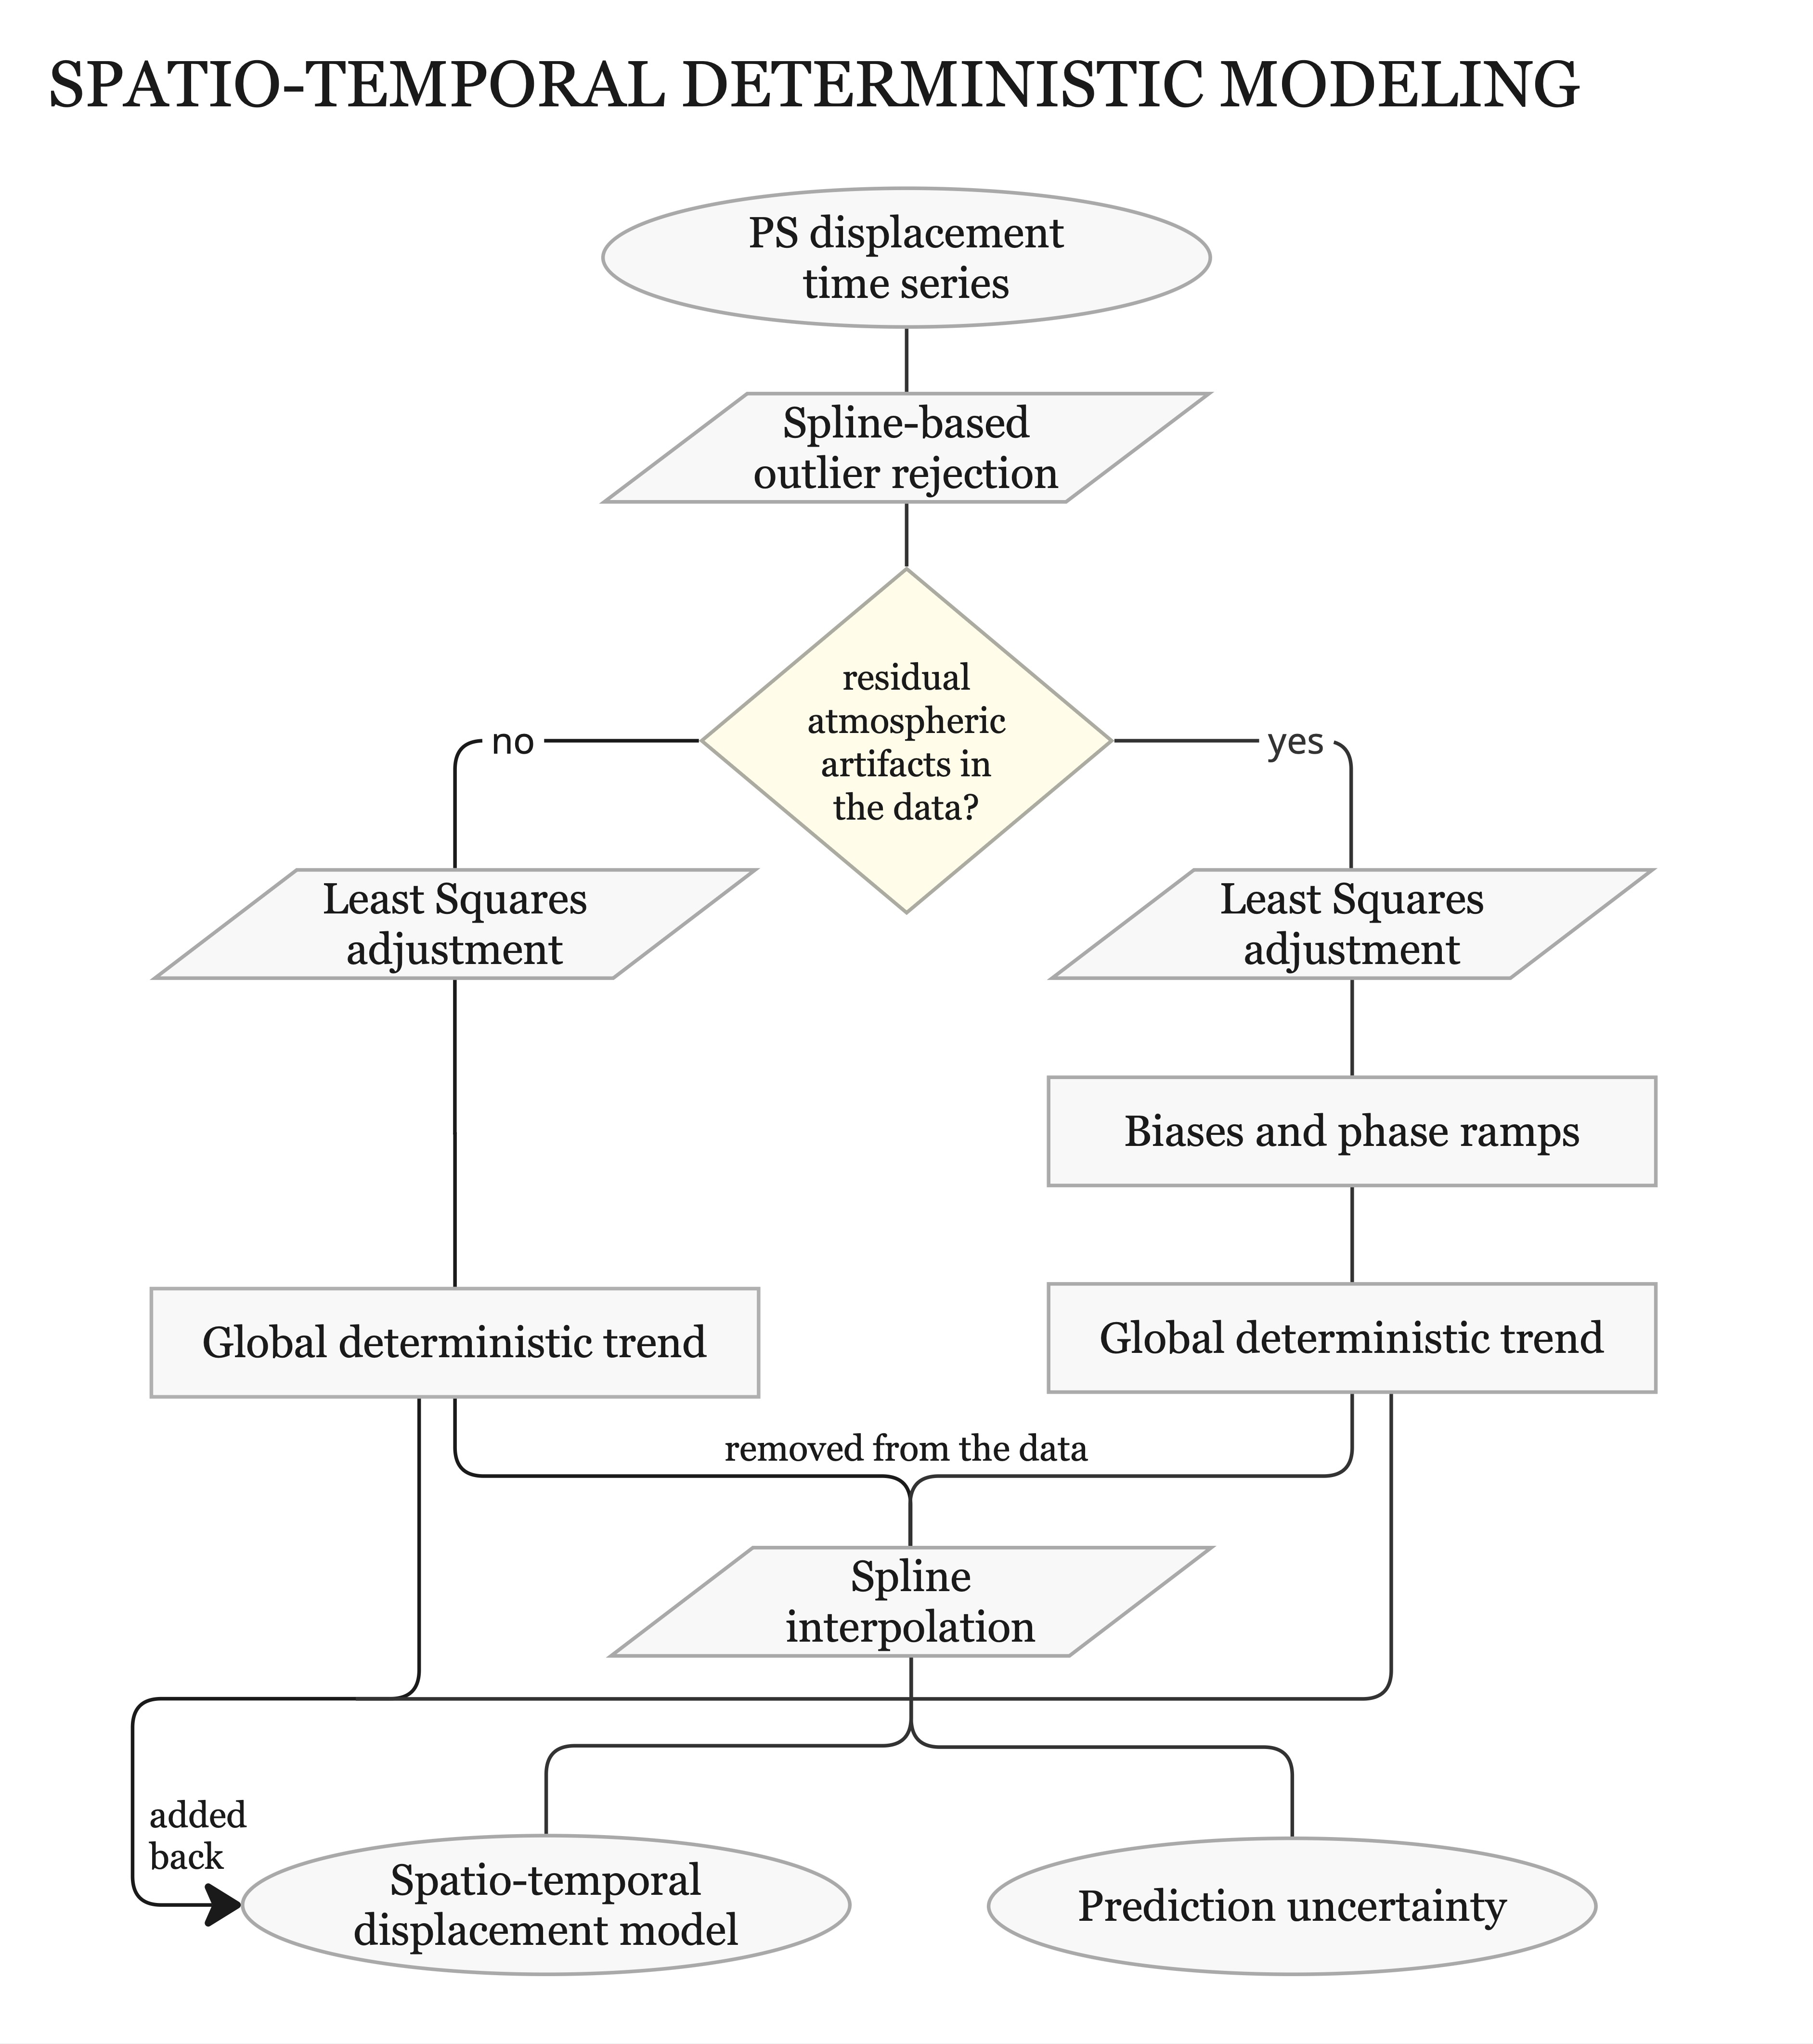
\includegraphics[width=1\textwidth]{images/G_ST_deterministic.jpg}
    \caption{Schematic representation of the deterministic spatio-temporal modeling workflow, progressing from raw PS observations through global polynomial trend removal and final multidimensional spline interpolation.}
    \label{fig:diag_det}
\end{figure}

\subsubsection{1D spatial domain}
Since the 1D infrastructure geometry involves one spatial dimension ($\ell$) and one temporal dimension ($t$), this mode fits a continuous surface using 2D bicubic splines. Configure it using the 1D deterministic controls.

Through this interface, you govern the specific estimators within the deterministic framework. Key configurable parameters include:
\begin{itemize}
    \item \textbf{Centerline and time resolution:} defines the uniform spatial ($\Delta \ell$) and temporal ($\Delta t$) step sizes for the target prediction grid upon which the final bicubic displacement surface is evaluated.
    \item \textbf{Minimum period for splines fitting:} establishes the maximum flexibility of the 1D splines used during the preliminary temporal outlier rejection step (structurally identical to the stochastic preprocessing).
    \item \textbf{Atmospheric residual errors:} if deemed present, these are estimated and removed. You can specify whether these errors are treated as purely time-variable biases (for small AOIs) or as epoch-specific spatial trends (for large AOIs).
    \item \textbf{Global trend:} defines the degree of a macroscopic spatio-temporal polynomial surface. Unlike the stochastic mode, this global surface is \textit{always} estimated and removed prior to the bicubic spline interpolation to ensure the splines only fit local, high-frequency physical deformations.
    \item \textbf{Bicubic spline optimization:} selects the strict statistical criteria (variance threshold, F-test, MDL or $\chi^2$ test) used to automatically determine the optimal number of spline knots for the final surface, preventing overfitting.
\end{itemize}

\subsubsection{2D spatial domain}
When the monitored AOI is a spatially distributed target (e.g., an urban center or a subsidence bowl), this module extends the deterministic, spline-based approach to the planar domain. It reconstructs the continuous deformation field $d(x,y,t)$ using 3D tricubic splines.

Selecting this option activates the 2D deterministic controls, which adapt the spatial resolution and optimization strategy to a planar grid.

The configuration parameters mirror those of the 1D deterministic case, adapted specifically for the expanded geometric domain. Most notably:
\begin{itemize}
    \item The \textbf{Spatial and time resolution} parameter now defines a uniform square grid spacing applied equally to both the Easting ($x$) and Northing ($y$) axes.
    \item The \textbf{Global trend} polynomial degree defines a trivariate surface instead of a bivariate one.
\end{itemize}


\subsection{Query points}
The filepath to a \texttt{.txt} file containing the coordinates (UTM or geographic) of query points can be specified in this last panel. This will trigger the interpolation module of the software to evaluate the estimated spatio-temporal model exactly at these coordinates. In the output Excel report this will result in displacement time series plots in the \textit{Interpolation} sheet.

Additionally, there is also a checkbox to export the modeled displacement time series at the observed PS positions. This can be found in the \textit{Modelled PS} sheet of the generated Excel report.


\section{Automatic report generation and data export}
To facilitate the interpretation and dissemination of the results, the software includes a fully automated workflow for report generation. Upon completion of the processing chain, the software aggregates the numerical results, the estimated statistical parameters, and the generated figures into a comprehensive Microsoft Excel spreadsheet.

The report is structured into five (or six/seven, if external interpolation and/or PS modeling is requested) specific sheets:

\subsection{General sheet}
This sheet serves as the project summary. It compiles all relevant metadata regarding the analysis, including:
\begin{itemize}
    \item \textbf{Project metadata:} date of execution, municipality, and country of the AOI (automatically geocoded from the reference PS point), and the chosen modeling strategy (e.g., 1D vs. 2D, stochastic vs. deterministic).
    \item \textbf{Input parameters:} details on the PS dataset, including the total number of scatterers, the observation period, and the unwrapping reference point coordinates. If available, the specific StaMPS processing parameters used in the upstream analysis are also reported.
    \item \textbf{Visual context:} three figures are automatically embedded: the project logo, a topographic map locating the AOI within the country, and a satellite map showing the distribution of PS points inside and outside the selected AOI (Figure~\ref{fig:sheet_general}).
\end{itemize}

\begin{figure}[H]
    \centering
    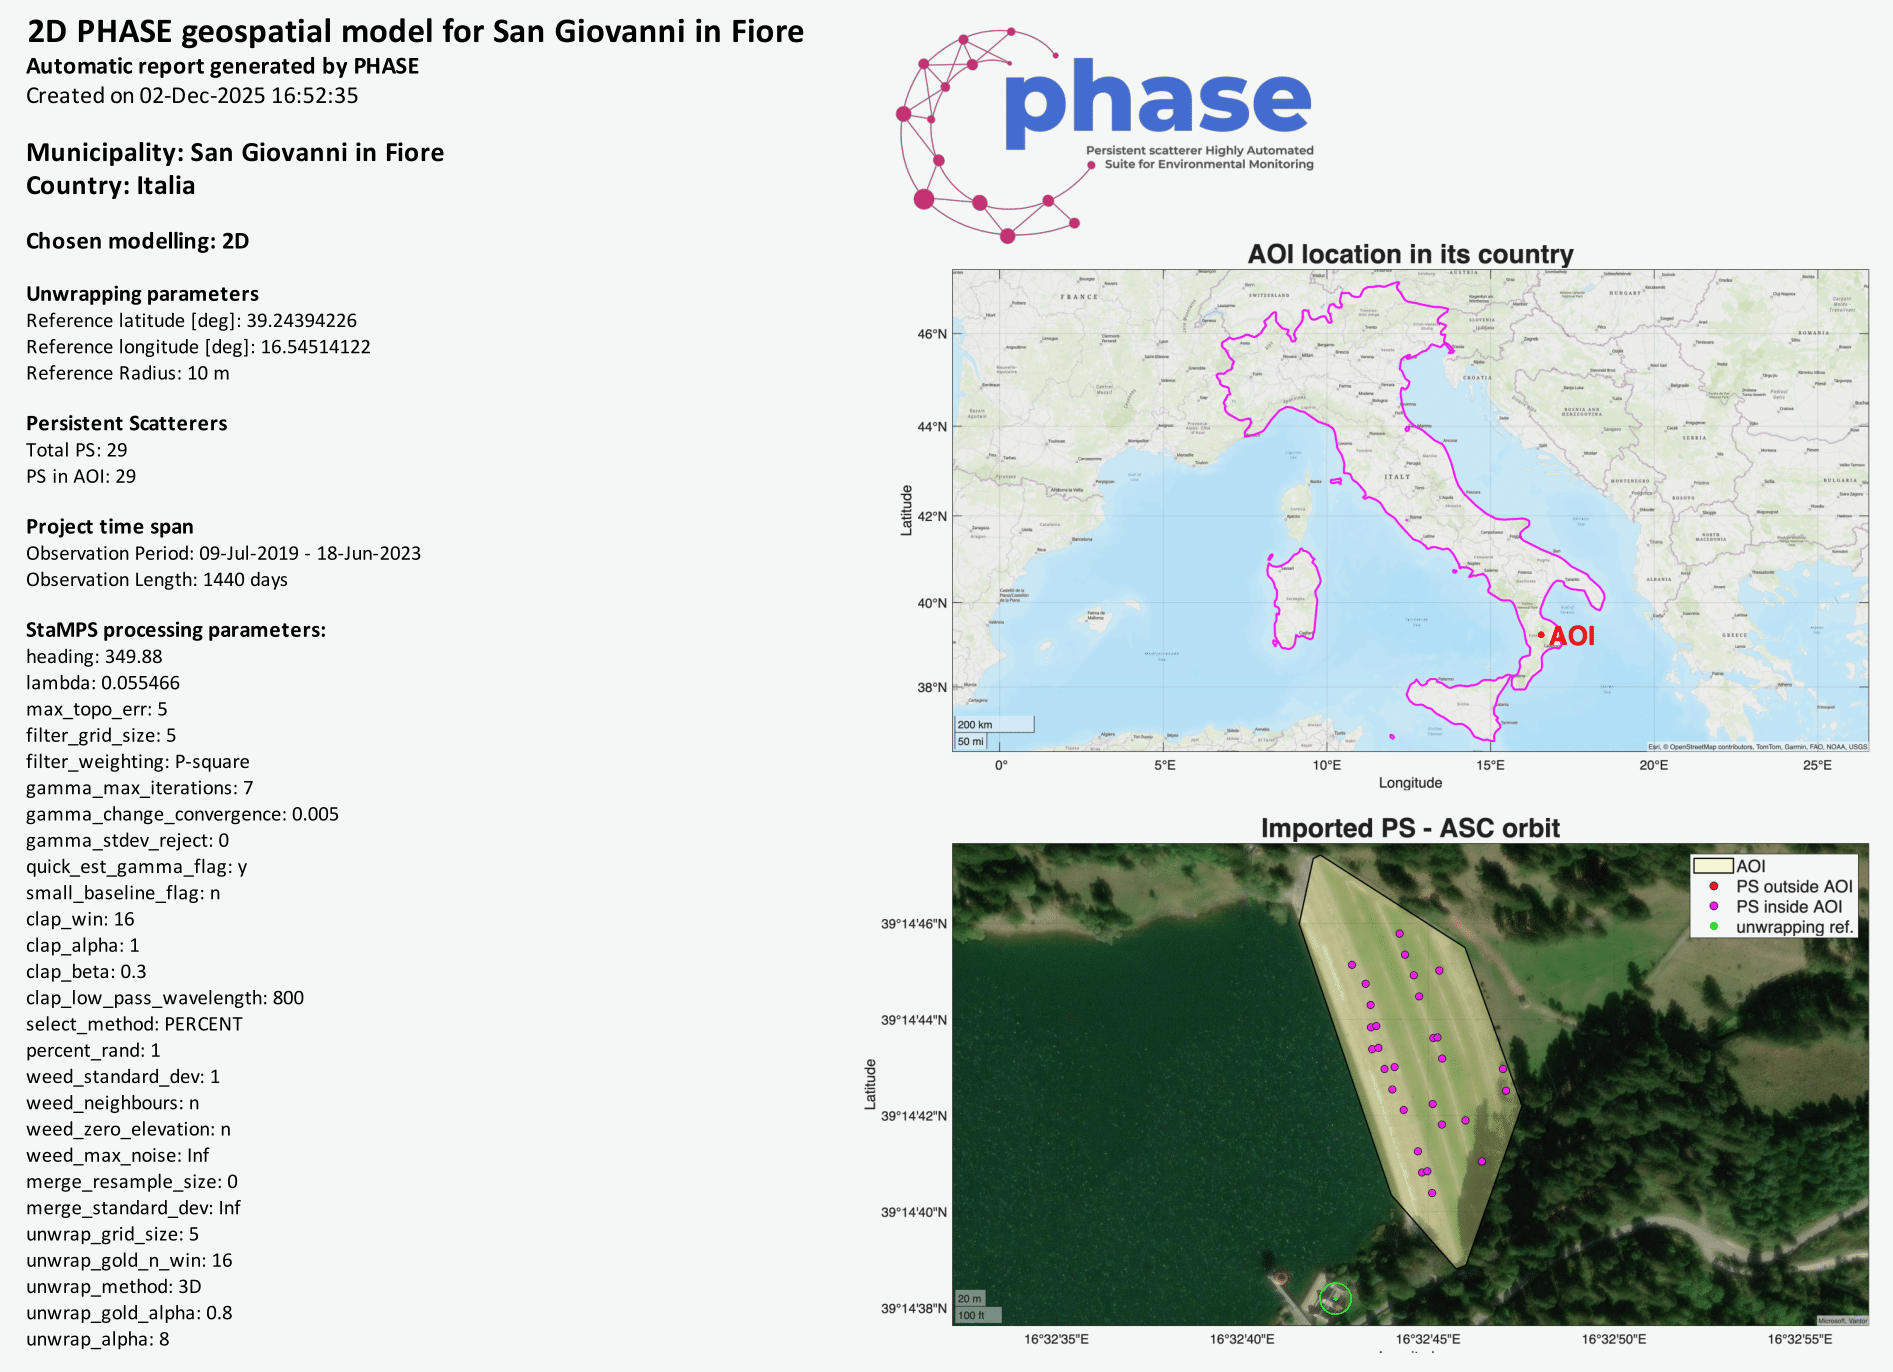
\includegraphics[width=0.9\textwidth]{images/sheet_general.png}
    \caption{Example of the \textit{General} sheet in the automatic output report, showing project metadata and context maps.}
    \label{fig:sheet_general}
\end{figure}

\subsection{Data sheets (Raw, Modeled, Uncertainty)}
Following the general overview, the core results are organized into three dedicated sheets. Each shares a similar structure: a header with summary statistics followed by the full data table, where rows represent individual PS points and columns represent observation epochs.

\begin{itemize}
    \item \textbf{Raw displacement:} contains the input PS time series after the initial detrending (subtraction of the modeled value at the first epoch). It includes a plot of the spatially averaged displacement time series over the AOI with an overlaid linear trend to identify macroscopic subsidence or uplift phenomena.
    \item \textbf{Modeled displacement:} contains the final result of the spatio-temporal modeling (stochastic or deterministic). It includes the full set of estimated displacement time series for all positions in the AOI based on the chosen spatial resolution. A map showing the average velocity (in mm/year) is embedded to provide an immediate overview of deformation rates (Figure~\ref{fig:sheet_modeled}).
    \item \textbf{Uncertainty:} mirroring the modeled displacement, this sheet reports the final-stage prediction standard deviation for every epoch and point, following the convention explained above. Its summary column and map show the arithmetic time mean of those standard deviations, not a propagated variance or an independent uncertainty estimate. This helps identify areas where predictions are less precise, for example near sparse PS coverage. In temporal-plus-NNI mode, the values at new grid locations are directly interpolated standard deviations; no interpolation covariance is propagated, so treat them as an uncertainty proxy rather than a rigorous prediction interval.
\end{itemize}

\begin{figure}[H]
    \centering
    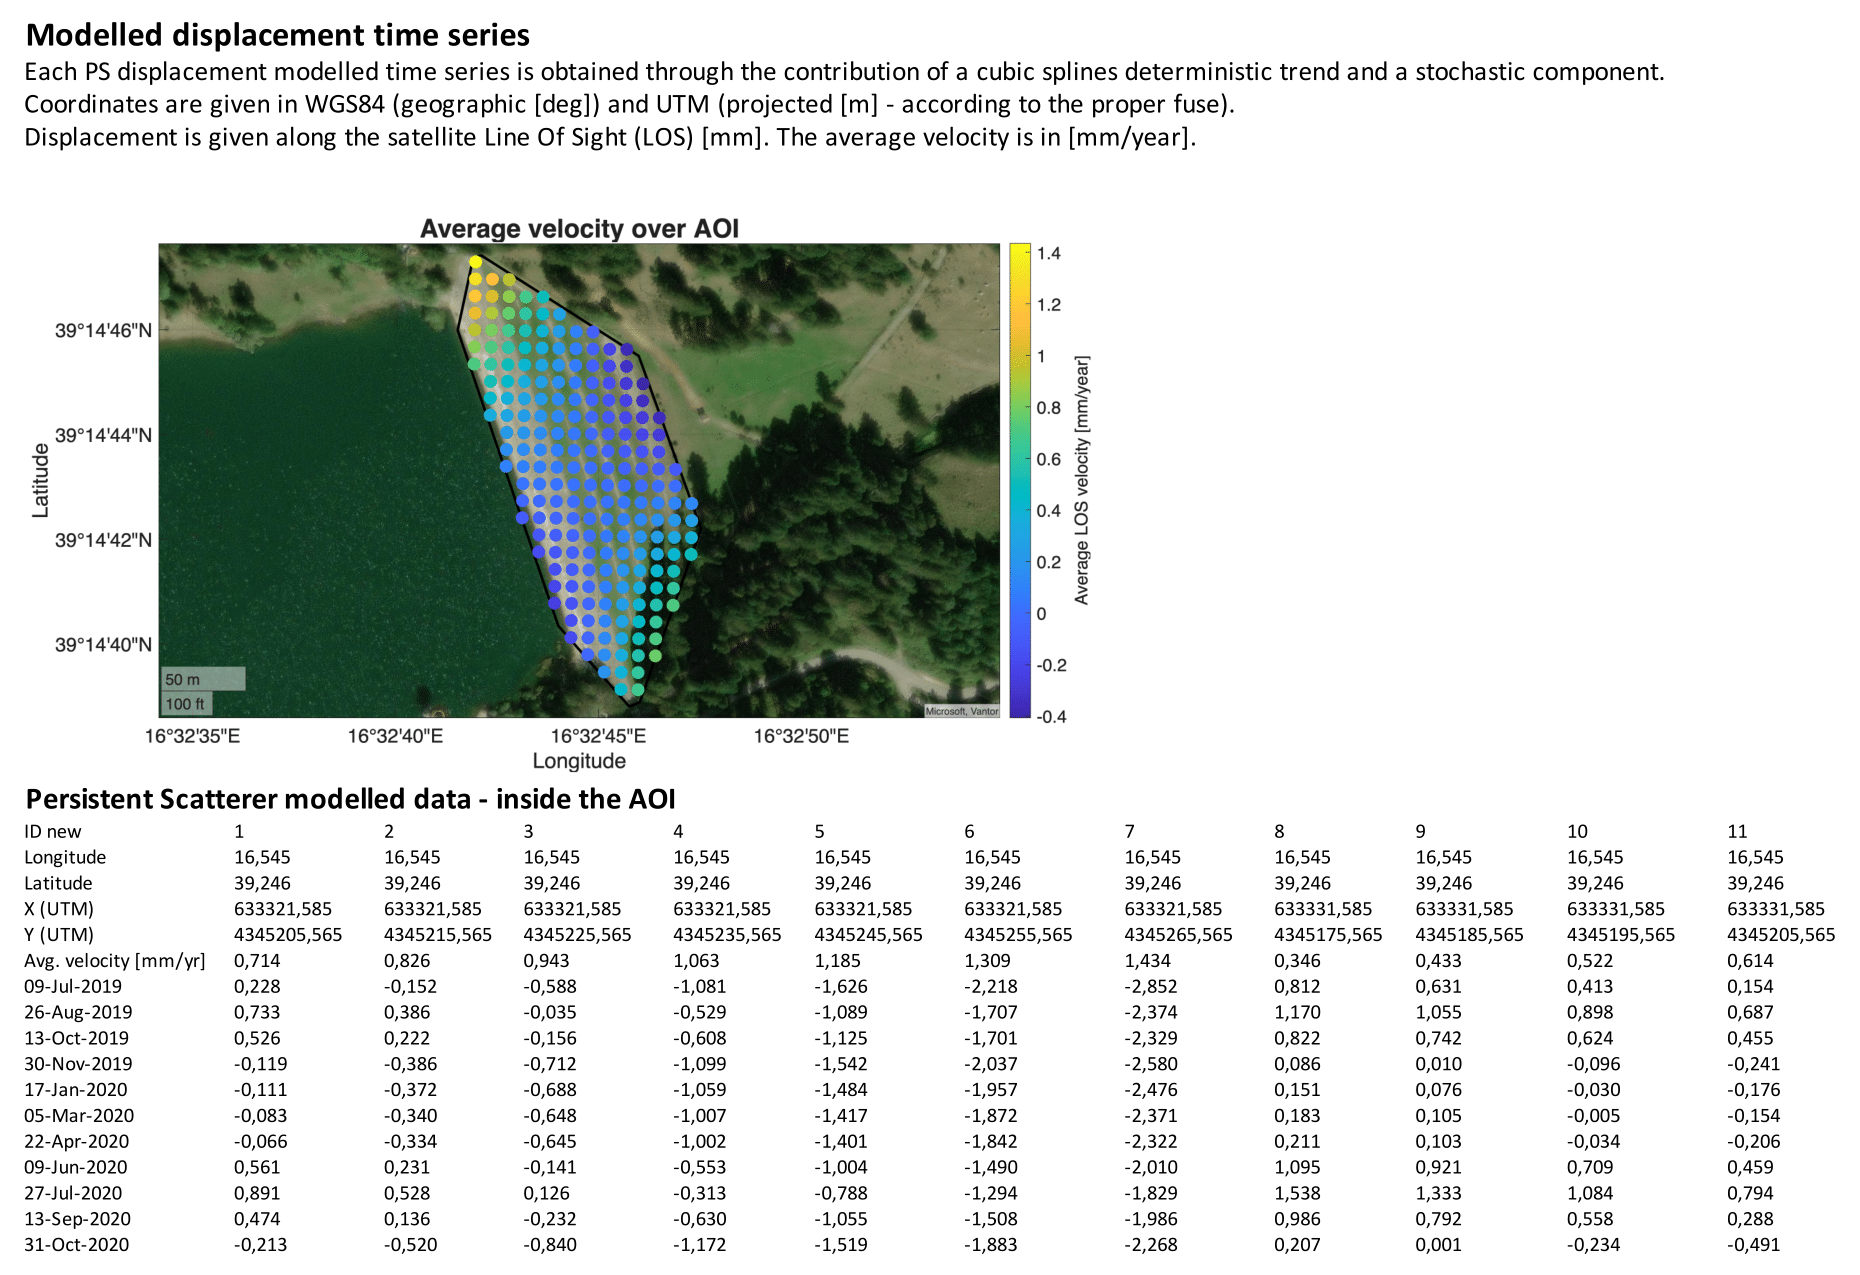
\includegraphics[width=0.9\textwidth]{images/sheet_modelled.png}
    \caption{Example of the \textit{Modeled displacement} sheet, featuring the data table and the average velocity map.}
    \label{fig:sheet_modeled}
\end{figure}

\subsection{Interpolation sheet (optional)}
If you provide a set of specific target coordinates (e.g., GNSS stations or critical infrastructure points), this sheet reports the displacement time series extracted from the continuous spatio-temporal model at those exact locations. This feature allows you to retrieve the deformation history at arbitrary points, regardless of the original PS distribution. For each target point, a specific plot showing the temporal evolution of the displacement is automatically generated and embedded.

\subsection{Modelled PS sheet (optional)}
If you flag this option, this sheet reports the displacement time series extracted from the continuous spatio-temporal model at the observed PS coordinates.

\subsection{AOI anomalies sheet (descriptive comparison)}
The \textit{AOI anomalies} sheet compares each complete \emph{modelled} LOS displacement series with the AOI median at each epoch. This highlights locations whose fitted deformation differs from the rest of the AOI without treating a noisy raw-observation residual as a deformation anomaly. For regularly spaced 1D centerlines or 2D grids, each modelled location has equal length or area weight in this comparison.

At each epoch $t$, the reference is the spatial median $m(t)$ of modelled displacement $\hat d_i(t)$. The robust AOI scale is $1.4826\,\operatorname{median}_i|\hat d_i(t)-m(t)|$, bounded below by the spatial median of the reported prediction standard deviations. The output lists the maximum absolute deviation in millimetres, the maximum deviation divided by this scale, and the fraction of epochs with normalized contrast at least three. A \textit{transient} or \textit{persistent} label requires two consecutive modelled epochs above that descriptive threshold; persistence of at least 20\% of epochs yields \textit{persistent}. Average velocity remains available as context, but does not determine the label. These scores are relative to the selected AOI and are neither hazard probabilities nor formal significance tests. Changing the AOI can change the reference and the labels.

\subsection{GIS and data export}
Finally, in addition to the Excel report, the software automatically exports the results in GIS-compatible formats to facilitate integration with other geospatial workflows:
\begin{itemize}
    \item \textbf{ESRI Shapefile (\texttt{.shp}):} a vector point file containing all points with their attributes (ID, coordinates, average velocity, time-mean prediction standard deviation and descriptive AOI-anomaly class/contrast) and the full displacement time series as additional columns (one for each date). A \texttt{.prj} file defines the output coordinates as WGS84.
    \item \textbf{MATLAB data (\texttt{.mat}):} a structure array containing the same data for advanced post-processing directly in MATLAB.
    \item \textbf{GeoTIFF (\texttt{.tif}):} a multi-band GeoTIFF file containing the georeferenced displacement and uncertainty maps at each query epoch.
\end{itemize}

These outputs summarize the PSI post-processing, providing ready-to-use data that can be immediately ingested into monitoring algorithms, decision-making chains, and research activities.
